\documentclass{article}
\usepackage[T1]{fontenc}
\usepackage{lmodern}
\usepackage{graphicx}
\usepackage{amsmath,amssymb}
\usepackage[a4paper,margin=2cm]{geometry}
\usepackage[absolute,overlay]{textpos}
\setlength{\TPHorizModule}{1mm}
\setlength{\TPVertModule}{1mm}
\usepackage[indonesian]{babel}
\usepackage{hyperref}
\setlength{\emergencystretch}{2em}
% unit: Halaman 45

\begin{document}

% === Halaman 45 (llm) ===

\vspace{170.48mm}

Sumber: William Stalling, Cryptography and Network Security\nOverview \& Chapter 1\n\vspace{60mm}
\begin{center}
\textbf{Active Attack: Interruption}
\end{center}

% deskripsi: Diagram ilustrasi serangan aktif berupa gangguan (Interruption), yang menunjukkan Bob mencoba mengirim pesan kepada Alice melalui Internet, namun pengiriman tersebut diblokir oleh penyerang bernama Darth.
% bbox normalisasi: [0.1780, 0.2220, 0.8230, 0.7960]
\begin{textblock*}{135.45mm}(37.38mm,65.93mm)
\noindent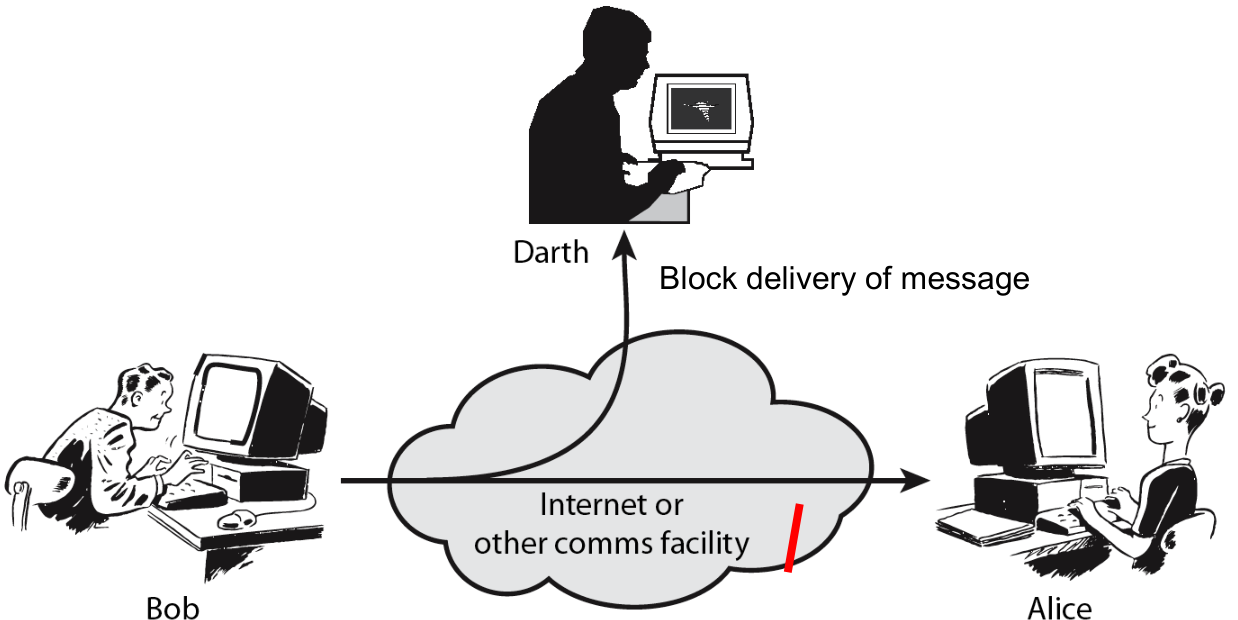
\includegraphics[width=135.45mm,height=170.48mm]{../../images/llm/page_045_img_01.png}%
\end{textblock*}

\end{document}
